% ============================================================================
% ARTIGO DO PROJETO DE APLICACAO | APRENDIZADO DE MAQUINA PARA SAUDE - UFF
% Projeto editavel no Overleaf: pdfLaTeX + BibTeX; citacoes ABNT autor-data.
% Todo o texto e ilustrativo. Substitua-o pelo conteudo real do projeto.
% O arquivo LEIA-ME.md apresenta orientacoes adicionais de escrita.
% ============================================================================
\documentclass[11pt,a4paper]{article}

% Idioma, caracteres e tipografia
\usepackage[T1]{fontenc}
\usepackage[utf8]{inputenc}
\usepackage[brazil]{babel}
\usepackage{lmodern}
\usepackage{microtype}
\usepackage{setspace}

% Pagina, estrutura e estilo
\usepackage[a4paper,top=2.55cm,bottom=2.5cm,left=2.75cm,right=2.65cm]{geometry}
\usepackage{xcolor}
\usepackage{titlesec}
\usepackage{fancyhdr}
\usepackage{graphicx}
\usepackage{booktabs}
\usepackage{tabularx}
\usepackage{array}
\usepackage{caption}
\usepackage{amsmath}
\usepackage{amssymb}
\usepackage{tikz}
\usetikzlibrary{positioning,arrows.meta}
\usepackage{enumitem}
\PassOptionsToPackage{hyphens}{url}
\usepackage[colorlinks=true,linkcolor=black,citecolor=azulescuro,urlcolor=azulescuro]{hyperref}
\usepackage[alf]{abntex2cite}
\urlstyle{same}

\definecolor{azulescuro}{RGB}{22,62,83}
\definecolor{cinzasec}{RGB}{96,107,115}
\definecolor{linha}{RGB}{213,221,224}
\definecolor{azulclaro}{RGB}{241,246,247}

\setstretch{1.12}
\setlength{\parindent}{1.25em}
\setlength{\parskip}{0.21em}
\setlength{\emergencystretch}{2em}
\captionsetup{font=small,labelfont=bf,justification=centering}
\titleformat{\section}{\large\sffamily\bfseries\color{azulescuro}}{\thesection}{0.70em}{}
\titleformat{\subsection}{\normalsize\sffamily\bfseries\color{azulescuro}}{\thesubsection}{0.65em}{}
\titlespacing*{\section}{0pt}{1.4em}{0.55em}
\titlespacing*{\subsection}{0pt}{1.05em}{0.35em}
\renewcommand{\refname}{Referências}
\addto\captionsbrazil{\renewcommand{\tablename}{Tabela}}
\setlength{\headheight}{14pt}
\pagestyle{fancy}
\fancyhf{}
\fancyhead[L]{\footnotesize\sffamily\color{cinzasec} APRENDIZADO DE MÁQUINA PARA SAÚDE}
\fancyhead[R]{\footnotesize\sffamily\color{cinzasec} UFF}
\fancyfoot[C]{\footnotesize\color{cinzasec}\thepage}
\renewcommand{\headrulewidth}{0.3pt}
\renewcommand{\footrulewidth}{0pt}
\fancypagestyle{plain}{\fancyhf{}\fancyfoot[C]{\footnotesize\color{cinzasec}\thepage}\renewcommand{\headrulewidth}{0pt}}

\newcommand{\aucA}{0,698}
\newcommand{\aucB}{0,898}
\newcommand{\fA}{0,661}
\newcommand{\fB}{0,842}
\newcommand{\recallA}{0,648}
\newcommand{\recallB}{0,852}
\newcommand{\aucAbl}{0,758}
\newcommand{\deltaAUC}{0,200}
\newcommand{\aucAlo}{0,629}
\newcommand{\aucAhi}{0,763}
\newcommand{\aucBlo}{0,858}
\newcommand{\aucBhi}{0,933}
\newcommand{\diffLo}{0,134}
\newcommand{\diffHi}{0,263}

\begin{document}

\begin{center}
  {\sffamily\footnotesize\color{azulescuro}\bfseries PROJETO DE APLICAÇÃO \enspace|\enspace ARTIGO CIENTÍFICO}\par
  \vspace{0.65em}
  {\LARGE\sffamily\bfseries Predição da busca por tratamento de saúde mental entre profissionais de tecnologia: comparação de modelos organizacionais e ampliados}\par
  \vspace{0.85em}
  {\normalsize Daniel Fontoura}\par
  \vspace{0.15em}
  {\small Instituto de Computação -- Universidade Federal Fluminense}\par
  {\small\color{cinzasec} Introdução ao Aprendizado de Máquina para Saúde \enspace|\enspace 2026.2}\par
  \vspace{0.85em}
  {\color{linha}\rule{\linewidth}{0.8pt}}
\end{center}
\vspace{-0.7em}

\begin{center}\textbf{\sffamily Resumo}\end{center}
\vspace{-0.85em}
\begin{quote}\small
Este estudo investiga se características e percepções do ambiente de trabalho de profissionais de tecnologia estão associadas à classificação retrospectiva da busca autorrelatada por tratamento de saúde mental. Foram analisadas 1.259 respostas da \textit{Mental Health in Tech Survey} de 2014, organizada pela Open Sourcing Mental Illness. Dois conjuntos de preditores foram comparados: (A) 18 variáveis organizacionais e de percepção do trabalho; e (B) as mesmas variáveis acrescidas de idade, gênero agrupado, histórico familiar e interferência percebida da saúde mental no trabalho. Foram treinados regressão logística, árvore de decisão e Random Forest com pré-processamento integrado ao ajuste, validação cruzada estratificada de cinco partições no treinamento e teste independente de 252 registros. O modelo organizacional selecionado obteve AUROC de \aucA\ e F1 de \fA; o ampliado alcançou AUROC de \aucB\ e F1 de \fB. Contudo, a análise de ablação sem \texttt{work\_interfere} reduziu a AUROC do modelo ampliado de regressão logística para \aucAbl. A ausência dessa resposta quase sempre coincidiu com não ter buscado tratamento, indicando importante efeito de informação condicional e possível atalho preditivo. Os resultados sugerem sinal associativo nas respostas organizacionais, mas não permitem inferir causalidade, realizar diagnóstico, antecipar busca futura ou justificar decisões individuais de recursos humanos.
\end{quote}
\vspace{-0.35em}
\noindent\textbf{Palavras-chave:} aprendizado de máquina; saúde mental; trabalho em tecnologia; busca por tratamento; classificação supervisionada.
\vspace{0.55em}

\section{Introdução}\label{sec:introducao}

A saúde mental no ambiente profissional envolve dimensões clínicas, sociais e organizacionais. Estigma, condições de suporte e percepções sobre a disposição para falar de sofrimento psicológico podem influenciar como trabalhadores expressam necessidades e acessam cuidados. Uma revisão sistemática sobre divulgação de problemas de saúde mental no trabalho identificou temas recorrentes relacionados ao estigma, ao contexto organizacional e à identidade profissional \cite{mcgrath2023disclosure}. Entretanto, a divulgação de um problema no trabalho e a busca por tratamento são comportamentos distintos, e resultados sobre um deles não podem ser automaticamente transferidos ao outro.

A Open Sourcing Mental Illness (OSMI) divulgou respostas da pesquisa \textit{Mental Health in Tech Survey} de 2014 para documentar experiências de profissionais do setor tecnológico com saúde mental e práticas do ambiente de trabalho \cite{osmi2014,osmi_research}. Os dados incluem informações sobre benefícios, suporte, possibilidade de afastamento, receios de consequências e histórico autorrelatado de procura de tratamento. Tal disponibilidade permite investigar padrões de classificação supervisionada, mas impõe cautela por se tratar de questionário voluntário, transversal e sem confirmação clínica do desfecho.

A pergunta deste estudo é: \textit{em que medida características e percepções organizacionais permitem discriminar, entre os respondentes da pesquisa, aqueles que relatam já ter buscado tratamento para uma condição de saúde mental?} Como objetivo secundário, investigamos o quanto atributos pessoais e relacionados à condição mental elevam o desempenho, em comparação com o conjunto estritamente organizacional. Esta comparação é importante porque usar um preditor associado diretamente ao histórico de sofrimento pode produzir excelente métrica sem responder à pergunta sobre o ambiente de trabalho.

O estudo contribui com um protocolo reprodutível, que evita ajustar transformações antes da divisão dos dados, compara três algoritmos, mede incerteza da AUROC e realiza ablação de uma variável condicional especialmente informativa. A organização dos métodos e dos resultados busca seguir recomendações de relato transparente de modelos preditivos, como o TRIPOD+AI \cite{collins2024tripodai}, sem caracterizar o presente exercício como modelo clínico validado.

\section{Trabalhos relacionados}\label{sec:relacionados}

\subsection{Levantamento e seleção da literatura}

Foi realizada leitura narrativa direcionada de fontes sobre o levantamento OSMI, saúde mental no trabalho e práticas de desenvolvimento e avaliação de modelos. Não se trata de revisão sistemática e não houve estratégia exaustiva de busca com estimativa de cobertura da literatura. O levantamento priorizou fontes primárias para caracterização do dataset e revisões pertinentes à interpretação ética e organizacional do fenômeno \cite{osmi2014,mcgrath2023disclosure,toth2023stigma}.

\subsection{Abordagens existentes e comparação crítica}

A revisão de \citeonline{mcgrath2023disclosure} sintetiza estudos sobre divulgação de problemas mentais no trabalho e destaca fatores como suporte, estigma e contexto da comunicação. Seu desfecho é divulgação, e não uso de tratamento; portanto, oferece fundamentação temática, mas não um parâmetro de AUROC diretamente comparável ao presente estudo. Já \citeonline{toth2023stigma} revisam evidências sobre intervenções para reduzir estigma relacionado à saúde mental em ambientes profissionais. Essa literatura ressalta a pertinência de intervenções e políticas coletivas, mas não autoriza inferir que uma variável associada no survey seja causa ou mecanismo de intervenção eficaz.

Do ponto de vista computacional, a comparação de regressão logística, árvores de decisão e florestas aleatórias permite estabelecer um contraste entre interpretabilidade e flexibilidade não linear \cite{pedregosa2011scikit,breiman2001rf}. A interpretação correta das curvas ROC demanda separar capacidade discriminativa de probabilidade calibrada e de acurácia em um limiar específico \cite{fawcett2006roc}. A importância por permutação, empregada neste trabalho, fornece diagnóstico associativo de atributos, mas não estimativas de efeito causal.

\subsection{Lacuna e posicionamento}

O objetivo não é demonstrar uma nova arquitetura de aprendizado, nem afirmar generalização populacional. A lacuna prática deste projeto é separar explicitamente a informação organizacional daquela potencialmente relacionada ao próprio histórico de tratamento, para verificar quanto da melhora aparente de desempenho decorre de uma característica autorrelatada condicional e potencialmente posterior ao desfecho.

\section{Materiais e métodos}\label{sec:metodos}

\subsection{Desenho do estudo e definição da tarefa}

Trata-se de análise secundária observacional e transversal de dados públicos, com tarefa de classificação binária supervisionada. A unidade de observação é a resposta de um participante, não um prontuário ou uma internação. A variável alvo \texttt{treatment} responde à pergunta \textit{``Have you sought treatment for a mental health condition?''}; mapeamos \texttt{Yes}=1 e \texttt{No}=0 \cite{osmi2014}. A classificação representa histórico informado no momento da pesquisa. Como os atributos do trabalho e a procura de tratamento foram observados no mesmo questionário, a ordenação temporal não é conhecida.

\subsection{Conjunto de dados e caracterização da amostra}\label{subsec:dados}

O arquivo \texttt{survey.csv} contém 1.259 respostas e 27 colunas. O alvo apresenta 637 respostas positivas (50,6\%) e 622 negativas (49,4\%). A pesquisa contempla múltiplos países, com predomínio dos Estados Unidos (751 respostas). Não se realizou amostragem probabilística para este estudo, nem foram aplicados critérios de exclusão de respondentes na análise preditiva.

A idade contém oito valores fora da faixa adulta plausível predefinida de 18 a 90 anos; foram substituídos por ausentes, preservando as 1.259 linhas. O campo \texttt{Gender} inclui 49 formas textuais diferentes, que foram agregadas conservadoramente em masculino, feminino e outra resposta/ambígua, sem inferir identidade nas categorias incertas. A falta de resposta de \texttt{work\_interfere} alcança 264 casos, o que merece análise independente devido à natureza condicional da pergunta. \texttt{comments}, \texttt{state} e \texttt{Timestamp} não foram usados como atributos. A coluna \texttt{Country} foi mantida apenas para caracterização exploratória de subgrupos.

\begin{figure}[htbp]
\centering
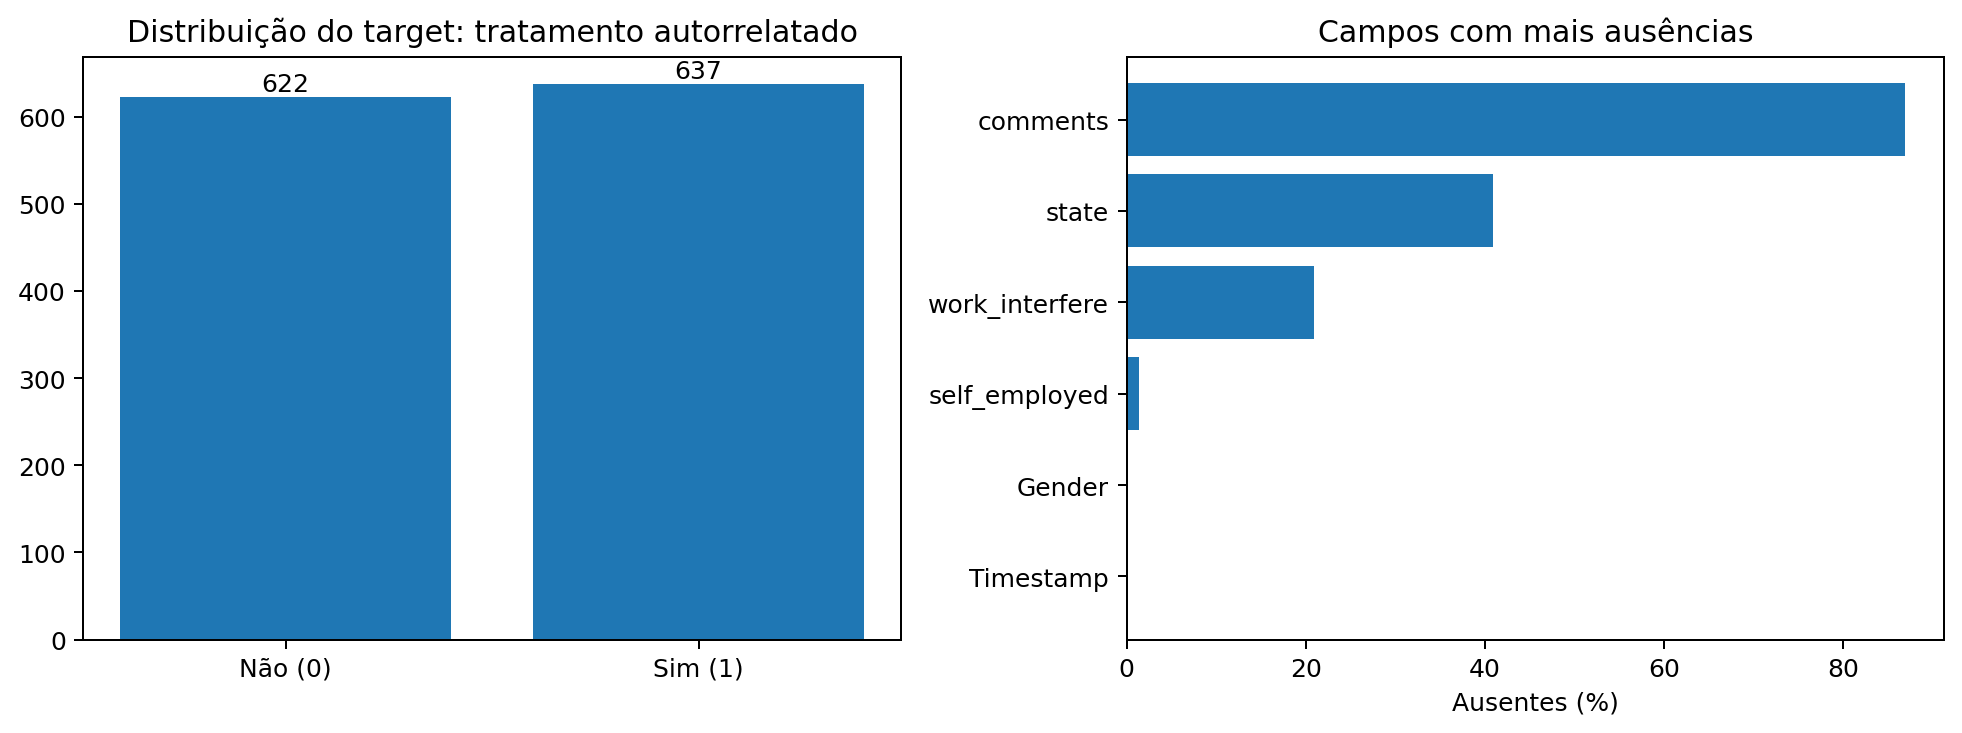
\includegraphics[width=0.94\linewidth]{figuras/01_eda_dataset.png}
\caption{Distribuição de \texttt{treatment} e padrões de ausência na base original.}
\label{fig:eda}
\par\vspace{3pt}{\footnotesize\color{cinzasec}Fonte: elaboração própria com dados da OSMI 2014.}
\end{figure}

\subsection{Conjuntos de atributos e preparação}

O conjunto A (organizacional) possui 18 variáveis: autoemprego, número de funcionários, trabalho remoto, tipo de empresa, benefícios, conhecimento de opções de atendimento, programa de bem-estar, recursos de apoio, anonimato, percepção de licença, consequências percebidas para saúde mental e física, disposição para falar com colegas e supervisores, disposição para discutir saúde em entrevistas, percepção de valorização da saúde mental e observação de consequências negativas. Elas abrangem tanto características declaradas das empresas como \textit{percepções individuais do ambiente}; não devem ser confundidas com indicadores objetivos auditados de políticas de RH.

O conjunto B acrescenta ao A quatro atributos: idade, gênero agrupado, histórico familiar e interferência percebida de condição mental no trabalho (\texttt{work\_interfere}). A última pergunta só é respondível de forma significativa por quem considera possuir tal condição. Para verificar o papel dessa variável, foi feita ablação excluindo apenas \texttt{work\_interfere}, mantendo as demais entradas do conjunto B.

Todas as transformações fazem parte de um \textit{Pipeline} do \textit{scikit-learn} \cite{pedregosa2011scikit}. A idade inválida é codificada como ausente e imputada com mediana ajustada no conjunto de treinamento do fold, seguida de padronização. Atributos categóricos recebem uma categoria explícita de não informado e codificação \textit{One-Hot}; categorias desconhecidas no teste são ignoradas. A ausência não foi substituída globalmente por moda antes da divisão dos dados, preservando a informação de não resposta.

\subsection{Formalização matemática e algoritmos}

Dado um vetor de atributos $\mathbf{x}_i$ e o rótulo $y_i\in\{0,1\}$, estimamos $\hat p_i=P(y_i=1\mid\mathbf{x}_i)$ e classificamos $\hat y_i=\mathbb{1}[\hat p_i\geq0{,}5]$. Na regressão logística, a probabilidade é modelada por:
\begin{equation}
\hat p_i=\frac{1}{1+\exp\left[-\left(\beta_0+\boldsymbol{\beta}^{\top}\mathbf{x}_i\right)\right]}.
\end{equation}
O treinamento utiliza regularização controlada pelo hiperparâmetro $C$. Para a árvore de decisão, partições são construídas pela minimização da impureza nos nós; a Random Forest agrega previsões de múltiplas árvores ajustadas a amostras e seleções de atributos aleatórias \cite{breiman2001rf}. Como referência ingênua, foi treinado um \textit{DummyClassifier} que atribui a todos a proporção positiva observada no treinamento; sua AUROC é 0,5.

\subsection{Validação, hiperparâmetros e prevenção de vazamento}

Os dados foram divididos uma única vez em treinamento (80\%, $n=1.007$, sendo 509 positivos) e teste (20\%, $n=252$, sendo 128 positivos), estratificados por alvo, com semente 42. Exclusivamente no treino, empregou-se validação cruzada estratificada com cinco folds e busca em grade por AUROC. Para regressão logística, $C\in\{0{,}1;1;10\}$; para a árvore, profundidade $\in\{3,5,8\}$ e mínimo de cinco amostras por folha; para a floresta, profundidade $\in\{6,12,\mathrm{ilimitada}\}$ com 180 árvores e mínimo de duas amostras por folha. O pré-processamento foi reestimado dentro de cada fold. A seleção do modelo representativo de cada experimento foi determinada pela AUROC média da validação cruzada, e não pelo desempenho de teste.

O teste, mantido reservado durante escolha de parâmetros, serviu à avaliação final. As métricas incluem AUROC, área sob a curva precisão--revocação (AUPRC), acurácia, precisão, sensibilidade (\textit{recall}) e F1. A sensibilidade e o F1 são calculados como
\begin{equation}
\operatorname{Recall}=\frac{VP}{VP+FN},\qquad
F1=\frac{2PR}{P+R},
\end{equation}
com $VP$ e $FN$ denotando verdadeiros positivos e falsos negativos, e $P$ e $R$ representando precisão e recall. Intervalos percentílicos exploratórios de 95\% para AUROC e para a diferença entre experimentos foram calculados com 1.000 reamostragens \textit{bootstrap} das observações de teste; a comparação da diferença é pareada. As curvas de aprendizado foram geradas com dados de treinamento via validação cruzada, sem reutilizar o teste para ajustar hiperparâmetros.

\subsection{Reprodutibilidade e aspectos éticos}

As bibliotecas empregadas incluem Python, pandas, NumPy, Matplotlib e scikit-learn. O repositório disponibiliza código, \textit{notebook}, sementes, hiperparâmetros, figura e tabelas agregadas. A cópia local do CSV não é versionada por padrão: o campo livre \texttt{comments} pode conter relatos sensíveis. O exercício não acessa essas respostas textuais e não é adequado a triagem de candidatos, vigilância de empregados ou classificação clínica individual. As recomendações TRIPOD+AI são utilizadas como referência de transparência, não como alegação de conformidade integral ou validação para uso em saúde \cite{collins2024tripodai}.

\section{Resultados}\label{sec:resultados}

\subsection{Caracterização e comparação do desempenho}

Nenhuma observação foi removida do experimento; oito idades foram imputadas após invalidar valores impossíveis. Os modelos de ambos os conjuntos utilizam o mesmo particionamento. A Tabela~\ref{tab:metricas} apresenta resultados do teste reservado.

\begin{table}[htbp]
\centering
\caption{Desempenho dos algoritmos no conjunto de teste ($n=252$).}
\label{tab:metricas}
\footnotesize
\setlength{\tabcolsep}{4pt}
\begin{tabular}{@{}llccccc@{}}
\toprule
\textbf{Grupo} & \textbf{Algoritmo} & \textbf{AUROC} & \textbf{AUPRC} & \textbf{Acurácia} & \textbf{Recall} & \textbf{F1}\\
\midrule
A & Regressão logística & 0,698 & 0,731 & 0,663 & 0,648 & 0,661\\
A & Árvore de decisão & 0,671 & 0,642 & 0,639 & 0,492 & 0,581\\
A & Random Forest & 0,708 & 0,735 & 0,651 & 0,602 & 0,636\\
\midrule
B & Regressão logística & 0,898 & 0,885 & 0,837 & 0,852 & 0,842\\
B & Árvore de decisão & 0,863 & 0,799 & 0,829 & 0,938 & 0,848\\
B & Random Forest & 0,883 & 0,857 & 0,798 & 0,828 & 0,806\\
\bottomrule
\end{tabular}
\par\vspace{3pt}{\footnotesize\color{cinzasec}Fonte: elaboração própria com base na OSMI 2014. Limiar 0,5; seleção por AUROC na validação cruzada.}
\end{table}


No conjunto A, a regressão logística obteve AUROC \aucA\ (IC95\% \aucAlo--\aucAhi), F1 \fA\ e sensibilidade \recallA. No conjunto B, a regressão logística obteve AUROC \aucB\ (IC95\% \aucBlo--\aucBhi), F1 \fB\ e sensibilidade \recallB. A diferença de AUROC B--A foi de \deltaAUC\ (IC95\% bootstrap pareado \diffLo--\diffHi). Embora a Random Forest tenha atingido AUROC ligeiramente maior no teste do conjunto A, a regressão logística foi escolhida com base no critério predefinido de validação cruzada, evitando selecionar retrospectivamente por resultado de teste.

\begin{figure}[htbp]
\centering
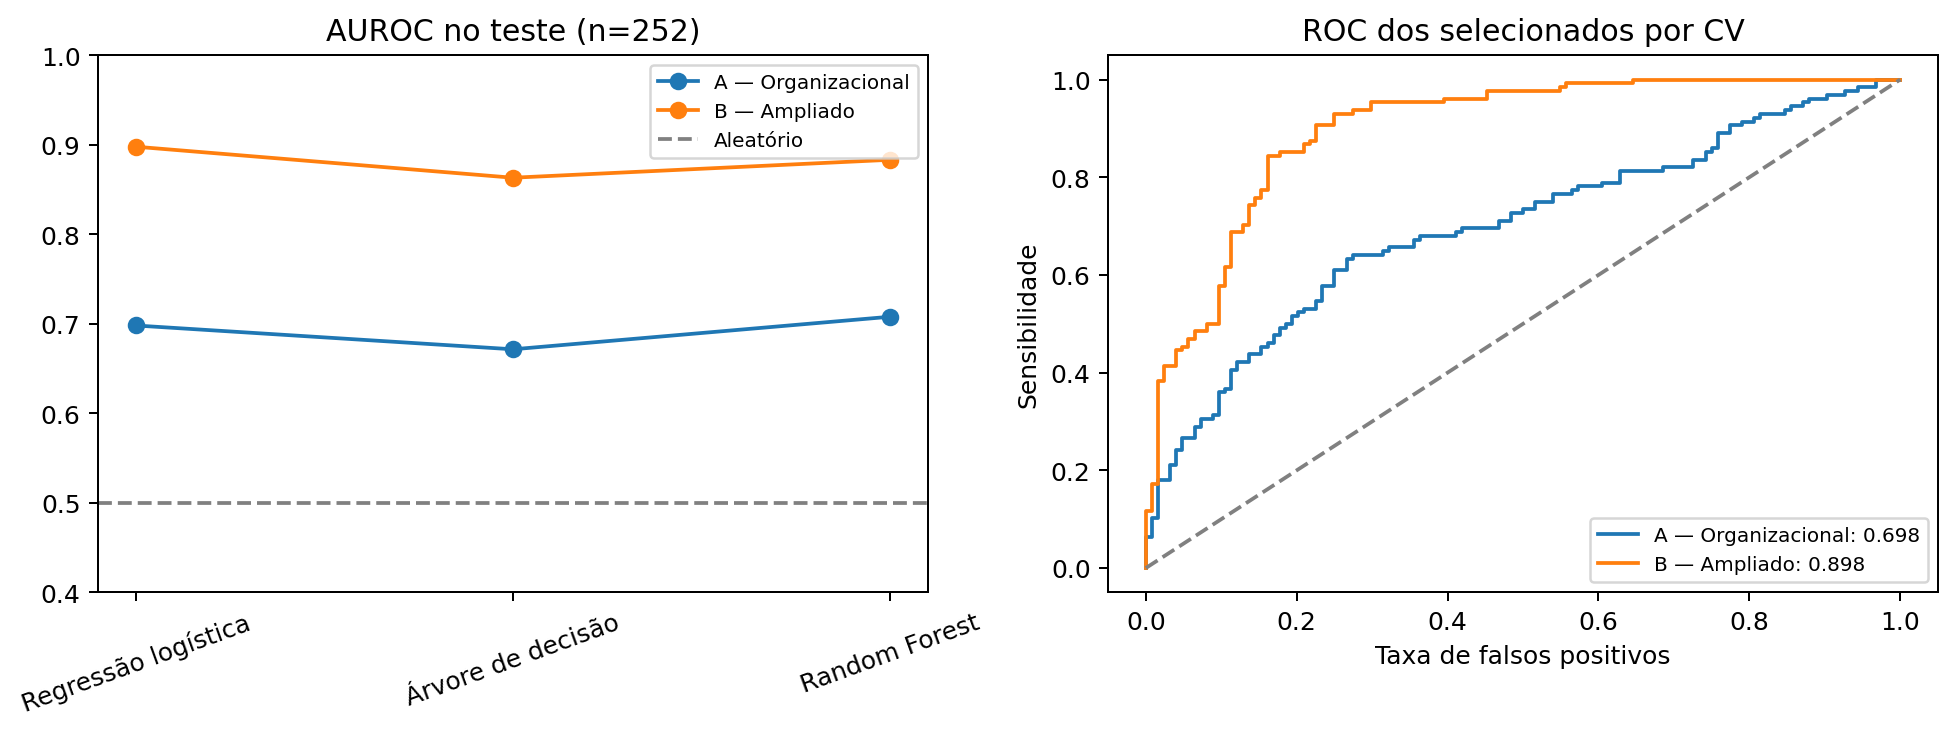
\includegraphics[width=0.92\linewidth]{figuras/02_modelos_roc.png}
\caption{AUROC por algoritmo e curvas ROC dos modelos selecionados na validação cruzada.}
\label{fig:roc}
\par\vspace{3pt}{\footnotesize\color{cinzasec}Fonte: elaboração própria; desempenho no conjunto reservado de teste.}
\end{figure}

\subsection{Análise de erros e ablação}

A matriz de confusão do conjunto A apresentou 83 verdadeiros positivos, 45 falsos negativos, 40 falsos positivos e 84 verdadeiros negativos. Para o B, houve 109 verdadeiros positivos, 19 falsos negativos, 22 falsos positivos e 102 verdadeiros negativos, no limiar fixo de 0,5. Esse ganho não constitui evidência de que características organizacionais tenham maior capacidade de indicar necessidade clínica de tratamento.

\begin{figure}[htbp]
\centering
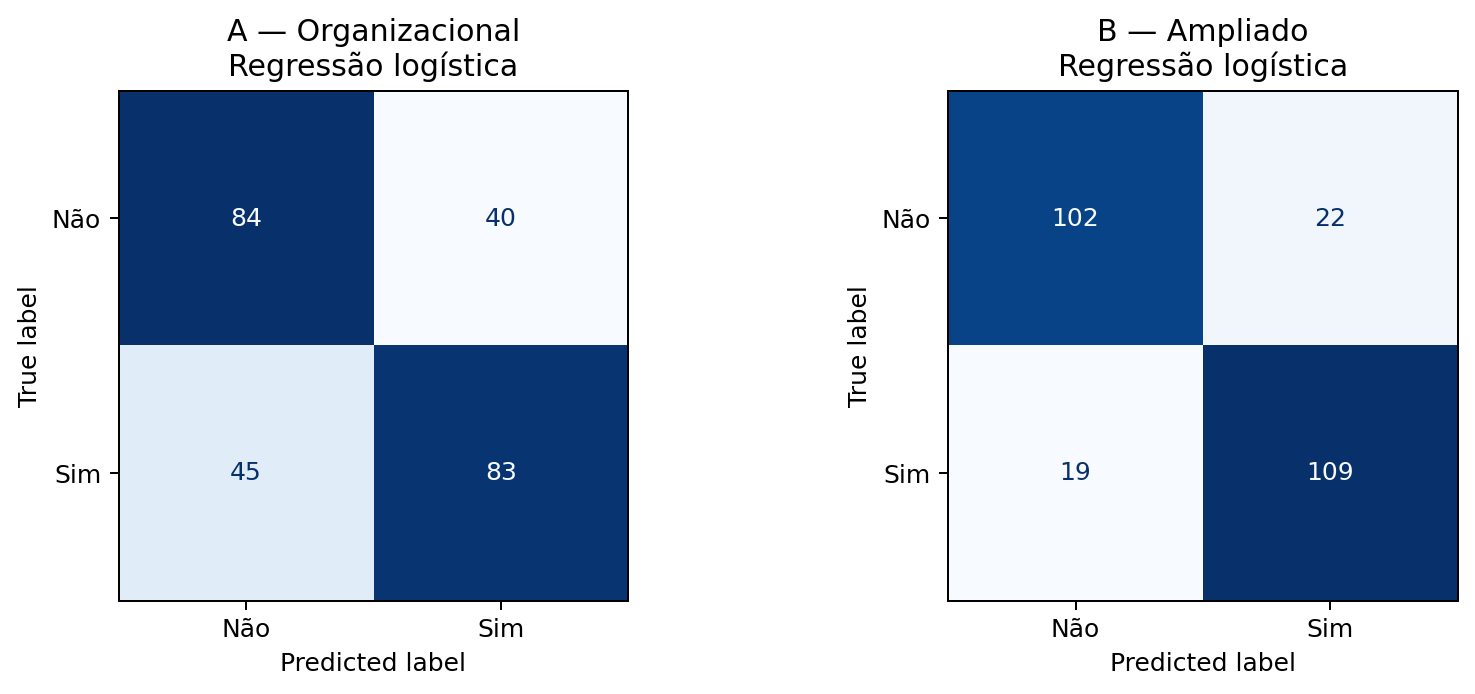
\includegraphics[width=0.88\linewidth]{figuras/03_matrizes_confusao.png}
\caption{Matrizes de confusão dos modelos selecionados (teste reservado).}
\label{fig:confusao}
\par\vspace{3pt}{\footnotesize\color{cinzasec}Fonte: elaboração própria.}
\end{figure}

O atributo \texttt{work\_interfere} apresenta um padrão de não resposta especialmente relevante: entre os 264 registros ausentes, 260 informaram \texttt{treatment=No} e apenas quatro informaram \texttt{treatment=Yes}. Quando se exclui essa única variável do conjunto ampliado, a regressão logística apresenta AUROC \aucAbl\ no teste, em vez de \aucB. A redução de aproximadamente 0,139 ponto indica que parte expressiva do desempenho ampliado dependia de uma pergunta condicional, cuja ausência por si só quase identifica a classe negativa. Isso recomenda interpretar a melhora como informação associativa próxima ao desfecho e não como solução superior para a pergunta organizacional.

\subsection{Curvas de aprendizado e importância por permutação}

As curvas de aprendizado da Figura~\ref{fig:aprendizado} representam AUROC de treinamento e validação em função da quantidade de exemplos disponíveis para ajuste. Elas não representam épocas de rede neural, pois os modelos comparados não foram redes treinadas por épocas. A análise de permutação da Figura~\ref{fig:importancia} indica, no conjunto A, relevância exploratória de conhecimento das opções de atendimento (\texttt{care\_options}) e benefícios; no B, \texttt{work\_interfere} passa a dominar a importância. A importância foi avaliada após o ajuste sobre o teste e não deve orientar nova seleção de atributos sem novo conjunto de validação.

\begin{figure}[htbp]
\centering
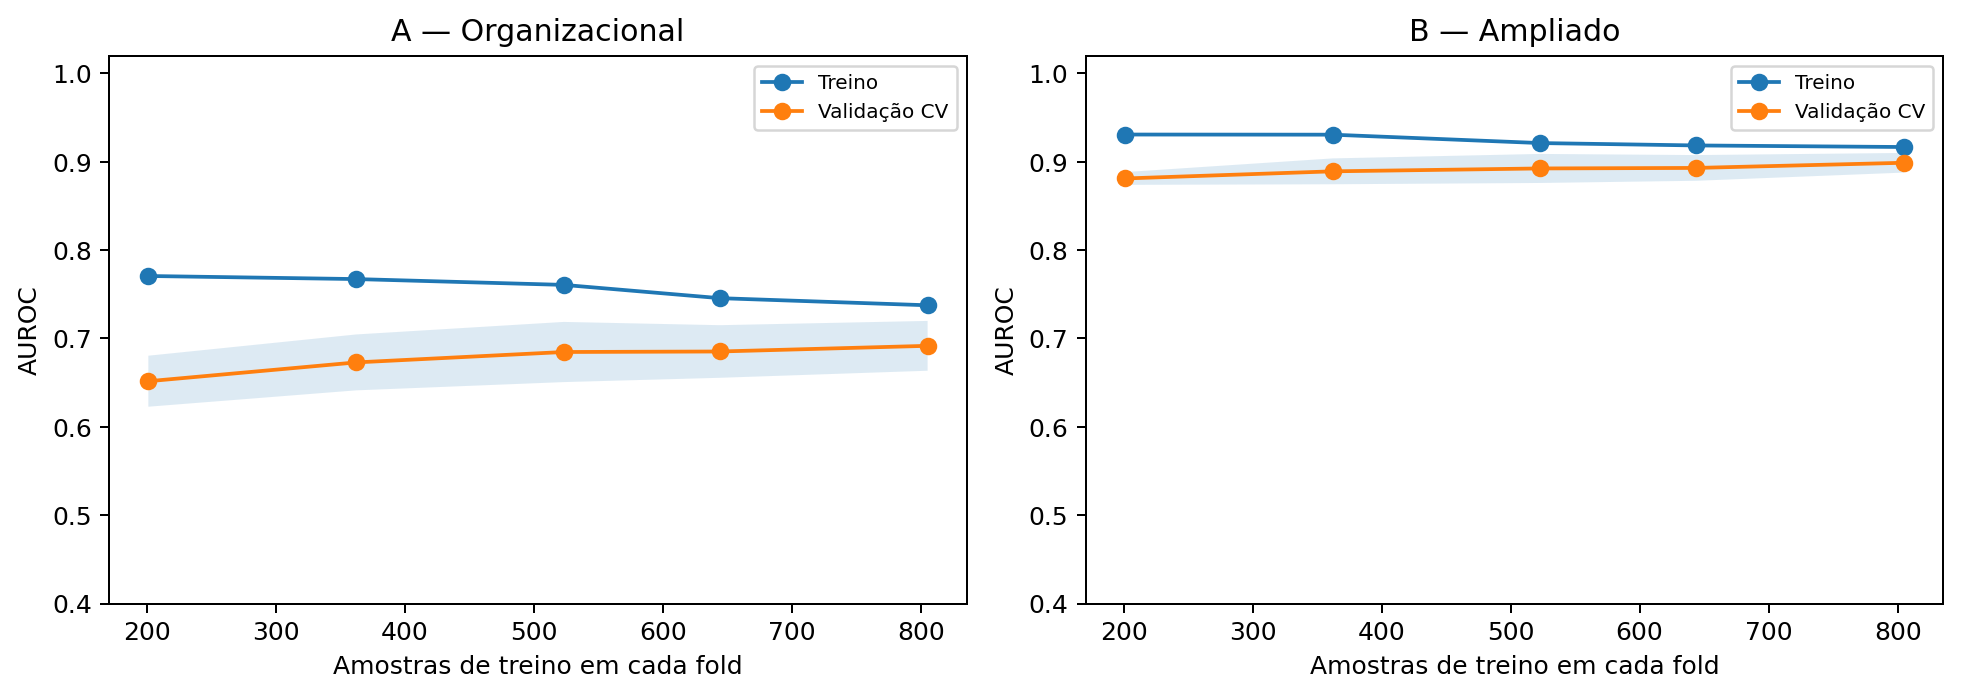
\includegraphics[width=0.93\linewidth]{figuras/04_curvas_aprendizado.png}
\caption{Curvas de aprendizado dos modelos selecionados, calculadas no treinamento por validação cruzada.}
\label{fig:aprendizado}
\par\vspace{3pt}{\footnotesize\color{cinzasec}Fonte: elaboração própria.}
\end{figure}

\begin{figure}[htbp]
\centering
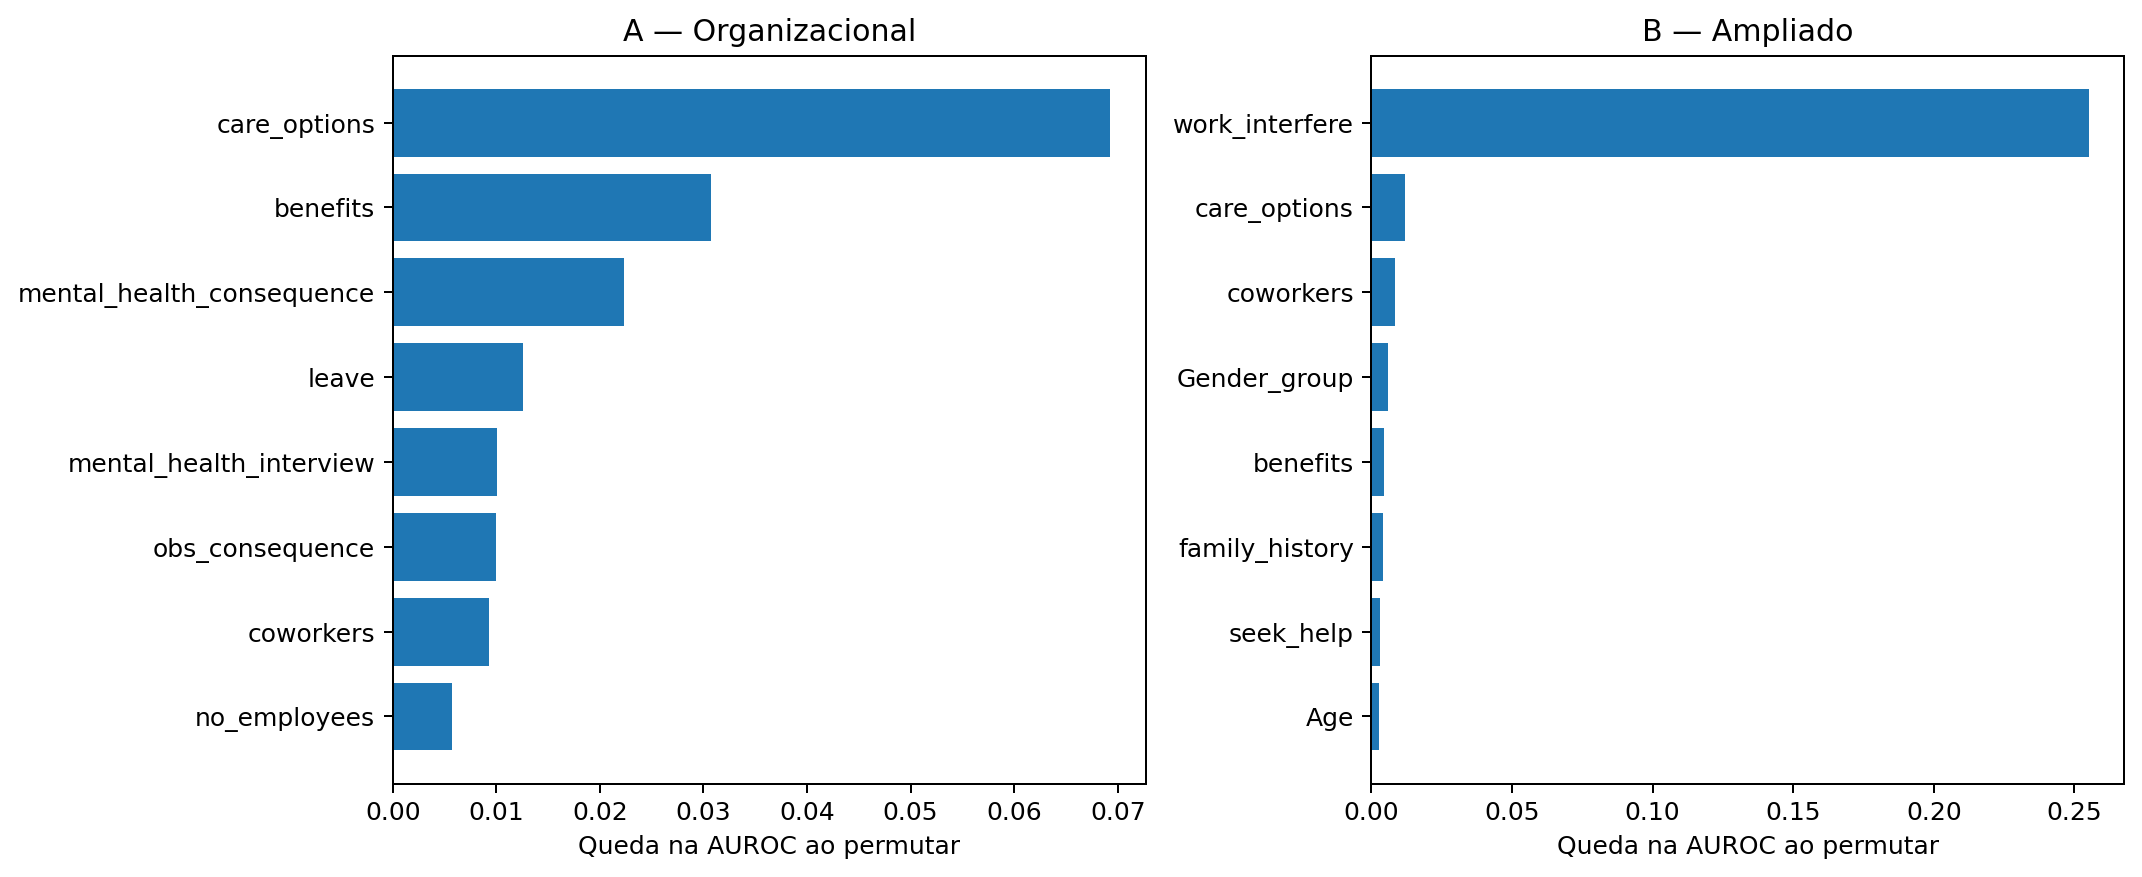
\includegraphics[width=0.94\linewidth]{figuras/05_importancia_permutacao.png}
\caption{Importância por permutação, medida como queda média na AUROC ao perturbar cada coluna original.}
\label{fig:importancia}
\par\vspace{3pt}{\footnotesize\color{cinzasec}Fonte: elaboração própria; análise exploratória no conjunto de teste.}
\end{figure}

\section{Discussão}\label{sec:discussao}

O modelo organizacional apresentou discriminação superior ao acaso, mas moderada. As respostas sobre serviços, suporte e atitudes no trabalho contêm informação sobre o histórico autorrelatado de tratamento entre participantes da OSMI 2014. Não se pode interpretar essa relação como evidência de que determinado benefício cause maior demanda clínica ou de que a retirada de um benefício reduza transtornos. A ausência de definição temporal torna plausível também a direção inversa: ter buscado tratamento pode alterar o conhecimento e a percepção do respondente sobre recursos disponíveis.

O resultado central é metodológico: a AUROC próxima de 0,90 obtida no conjunto ampliado seria enganosa se reportada isoladamente. A variável \texttt{work\_interfere} pergunta sobre interferência percebida de uma condição mental no trabalho e contém um padrão de ausência quase determinístico da classe negativa. A ablação revela que o resultado elevado está ligado a um sinal informativo que não pertence propriamente ao ambiente organizacional. A literatura sobre estigma e divulgação no trabalho apoia a relevância do tema, mas não valida essa variável como marcador clínico ou de decisão de RH \cite{mcgrath2023disclosure,toth2023stigma}.

Entre as limitações, destacam-se a amostragem não probabilística, o predomínio geográfico dos EUA, a coleta em 2014, a falta de identificador para verificar respostas duplicadas, a dependência de autorrelato, o agrupamento redutor de categorias de gênero, os campos condicionais e a ausência de confirmação clínica. O hold-out é interno à mesma fonte, e os intervalos bootstrap não incluem incerteza de seleção e treinamento de modelos. As métricas não indicam calibração clínica, utilidade prospectiva ou desempenho na população geral de profissionais de tecnologia. A existência de risco de estigmatização e discriminação torna inadequada sua aplicação à classificação individual de trabalhadores.

Como trabalhos futuros, recomenda-se validação temporal e externa com questionários comparáveis, investigação da robustez sem atributos potencialmente posteriores ao desfecho, análise de subgrupos com tamanho adequado, comparação de calibração e eventual formulação prospectiva com definição explícita do momento da previsão. Para RH, uma aplicação menos arriscada seria análise agregada e voluntária de conhecimento sobre benefícios e barreiras organizacionais, sem identificar ou pontuar pessoas.

\section{Conclusão}\label{sec:conclusao}

O estudo implementou e avaliou de forma reprodutível três algoritmos em dois cenários de atributos. Com respostas organizacionais, a regressão logística selecionada por validação cruzada alcançou AUROC \aucA; com atributos individuais, AUROC \aucB. Entretanto, a sensibilidade à exclusão de \texttt{work\_interfere} evidenciou a dependência de um preditor condicional e próximo ao histórico de tratamento, cuja presença pode distorcer a interpretação do ganho. Assim, o principal resultado científico do projeto não é a maior métrica isolada, mas a identificação das condições e limitações sob as quais ela foi produzida. A análise responde à pergunta de classificação retrospectiva na amostra observada, não estabelece causalidade e não sustenta uso clínico ou decisão individual sobre empregados.

\bibliography{referencias}
\end{document}
